\subsection{Data Fetching and Feature Extraction}
\label{subsec:results_data}

The results section commences with the presentation of Table~\ref{tab:records}, which summarizes the data retrieval phase.
Displayed within are the total records obtained from both databases, along with the corresponding total and median values extracted.

\begin{table}
    \renewcommand{\arraystretch}{1.5}
    \setlength{\tabcolsep}{12pt}
    \begin{center}
        \begin{tabular}{ |c|c|c| }
            \hline
            & MIMIC-III  & MIMIC-IV  \\
            \hline
            Records       & 22,083     & 5,508     \\
            \hline
            Total Values  & 13,659,375 & 1,309,265 \\
            \hline
            Median Values & 1,918,623  & 183,140   \\
            \hline
        \end{tabular}
    \end{center}
    \captionsetup{format=plain, justification=centering}
    \caption{Fetched and Extracted Data from MIMIC-III and MIMIC-IV DBs}
    \label{tab:records}
\end{table}

In a brief summary of the table data, 5,508 records were retrieved from the MIMIC-IV database, each encompassing 37,795 values, equating to approximately 605 seconds of data (at a sampling rate of 64.4725).
Conversely, a total of 22,083 records were obtained from the MIMIC-IV dataset, representing four times the number of records in comparison to MIMIC-IV\@.
Each of these records consisted of 75,625 values, likewise corresponding to an approximate duration of 10 minutes (with a sampling rate of 125).

Conversely, 4 times the records of MIMIC-IV were fetched, namely 22,083, each containing 75625 values also corresponding to approx.\ 10 minutes (sampling rate of 125).

Subsequently, the process of Feature Extraction from both DBs commenced, involving the extraction of 34 training features along with their corresponding values from the PPG waveforms,
as well as the target reference values for SBP, DBP, and MAP from the ABP signal.

From the MIMIC-IV dataset, a total of 1,309,265 values were extracted, leading to the creation of 34 x 1,309,265 PPG and 3 x 1,309,265 ABP data matrices.
Additionally, 183,140 median values were derived from these matrices, forming datasets of the same X-axis dimensions.
This set of data was utilized for the validation phase.

In the case of the MIMIC-III dataset, a total of 13,659,375 values were extracted, resulting in 34 x 13,659,375 PPG and 3 x 13,659,375 ABP data matrices.
Similarly, 1,918,623 median values were obtained from these matrices, creating datasets with identical X-axis structures.
These datasets were employed for the purposes of training and testing.

The data flow is visualized in Figure~\ref{fig:data_flow}.

\begin{figure}[h]
    \centering
    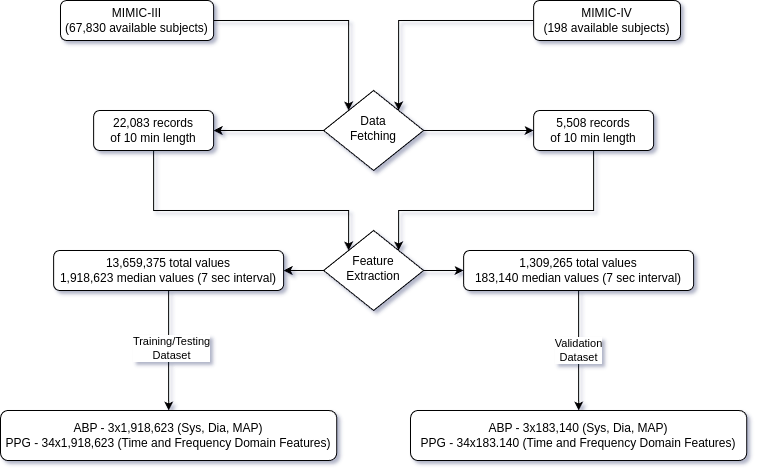
\includegraphics[width=0.9\textwidth]{images/results/flow_diagram}
    \caption{Flow Diagram presenting the Data Fetching and Processing}
    \label{fig:data_flow}
\end{figure}

\subsection{Machine Learning}
\label{subsec:machine_learning}

Moving on to the results from the ML phase, firstly the feature data preparation is elaborated.

As mentioned in previous chapters, an ideal ratio of 60/20/20 train/test/validate was aimed for.
However in the end having 1,918,623 values from MIMIC-III and 183,140 values from MIMIC-IV, we had to settle for a different splitting ratio.
As mentioned, the MIMIC-III data was used for training/testing, and it was split into 80/20 train/test, resulting in 1,534,898 training and 383,725 testing datapoints.
Therefore final train/test/validate proportions were:

\begin{center}
    \begin{tabular}{|c|c|c|}
        \hline
        Training  & Testing & Validation \\
        \hline
        1,534,898 & 383,725 & 183,140    \\
        \hline
        73\%      & 18\%    & 9\%        \\
        \hline
    \end{tabular}
\end{center}

% possibly discussion
All this means is that the signal processing algorithms worked better and extracted more values from the MIMIC-III DB.
It is also possible a hint at the fact, that the quality of the signal was better in MIMIC-III.
This is also logical however, since there was no limit on the fetching of records from a single study or subject from MIMIC-IV,
so huge number of segments might have been discarded, if they didn't showcase a comprehensible signal.

\begin{center}
    \begin{tabular}{ |c|c|c|c| }
        \hline
        & Training Loss (MSE) & Testing Loss (MSE) & Testing MAE \\
        \hline
        LR                     & 218.443             & -                  & 11.097      \\
        \hline
        MLP                    & 208.343             & -                  & 10.866      \\
        \hline
        LSTM                   & 93.81               & 97.358             & 6.953       \\
        \hline
        LSTM (weight adjusted) & 97.615              & 100.498            & 7.085       \\
        \hline
        Bi-LSTM                & -                   & -                  & -           \\
        \hline
        GRU                    & 88.34               & 92.142             & 6.759       \\
        \hline
        GRU (weight adjusted)  & 88.167              & 90.955             & 6.727       \\
        \hline
        Bi-GRU                 & -                   & -                  & -           \\
        \hline
        SVR                    & -                   & -                  & -           \\
        \hline
        RF                     & -                   & -                  & -           \\
        \hline
    \end{tabular}
\end{center}

\begin{center}
    \begin{tabular}{ |c|c|c|c| }
        \hline
        & Testing RMSE & Validation RMSE & Validation MAE \\
        \hline
        LR                     & 14.777       &                 &                \\
        \hline
        MLP                    & 14.446       &                 &                \\
        \hline
        LSTM                   & 9.866        & -               & 14.597         \\
        \hline
        LSTM (weight adjusted) & 10.024       & -               & 14.646         \\
        \hline
        Bi-LSTM                & -            & -               & -              \\
        \hline
        GRU                    & 9.598        & -               & 14.951         \\
        \hline
        GRU (weight adjusted)  & 9.536        & -               & 15.205         \\
        \hline
        Bi-GRU                 & -            & -               & -              \\
        \hline
        SVR                    & -            & -               & -              \\
        \hline
        RF                     & -            & -               & -              \\
        \hline
    \end{tabular}
\end{center}

LSTM \& GRU training and testing loss charts (32 \& 33) % (\ref{fig:train_mse} \& \ref{fig:test_mse}).

It was found, that every feature contributes positively, therefore feature reduction was not applied.
Feature Importance chart in Figure~34 (at the end of the document) % \ref{fig:feat_importance} (at end of document).

%\begin{figure}
%    \centering
%    \begin{subfigure}{0.5\textwidth}
%        \centering
%        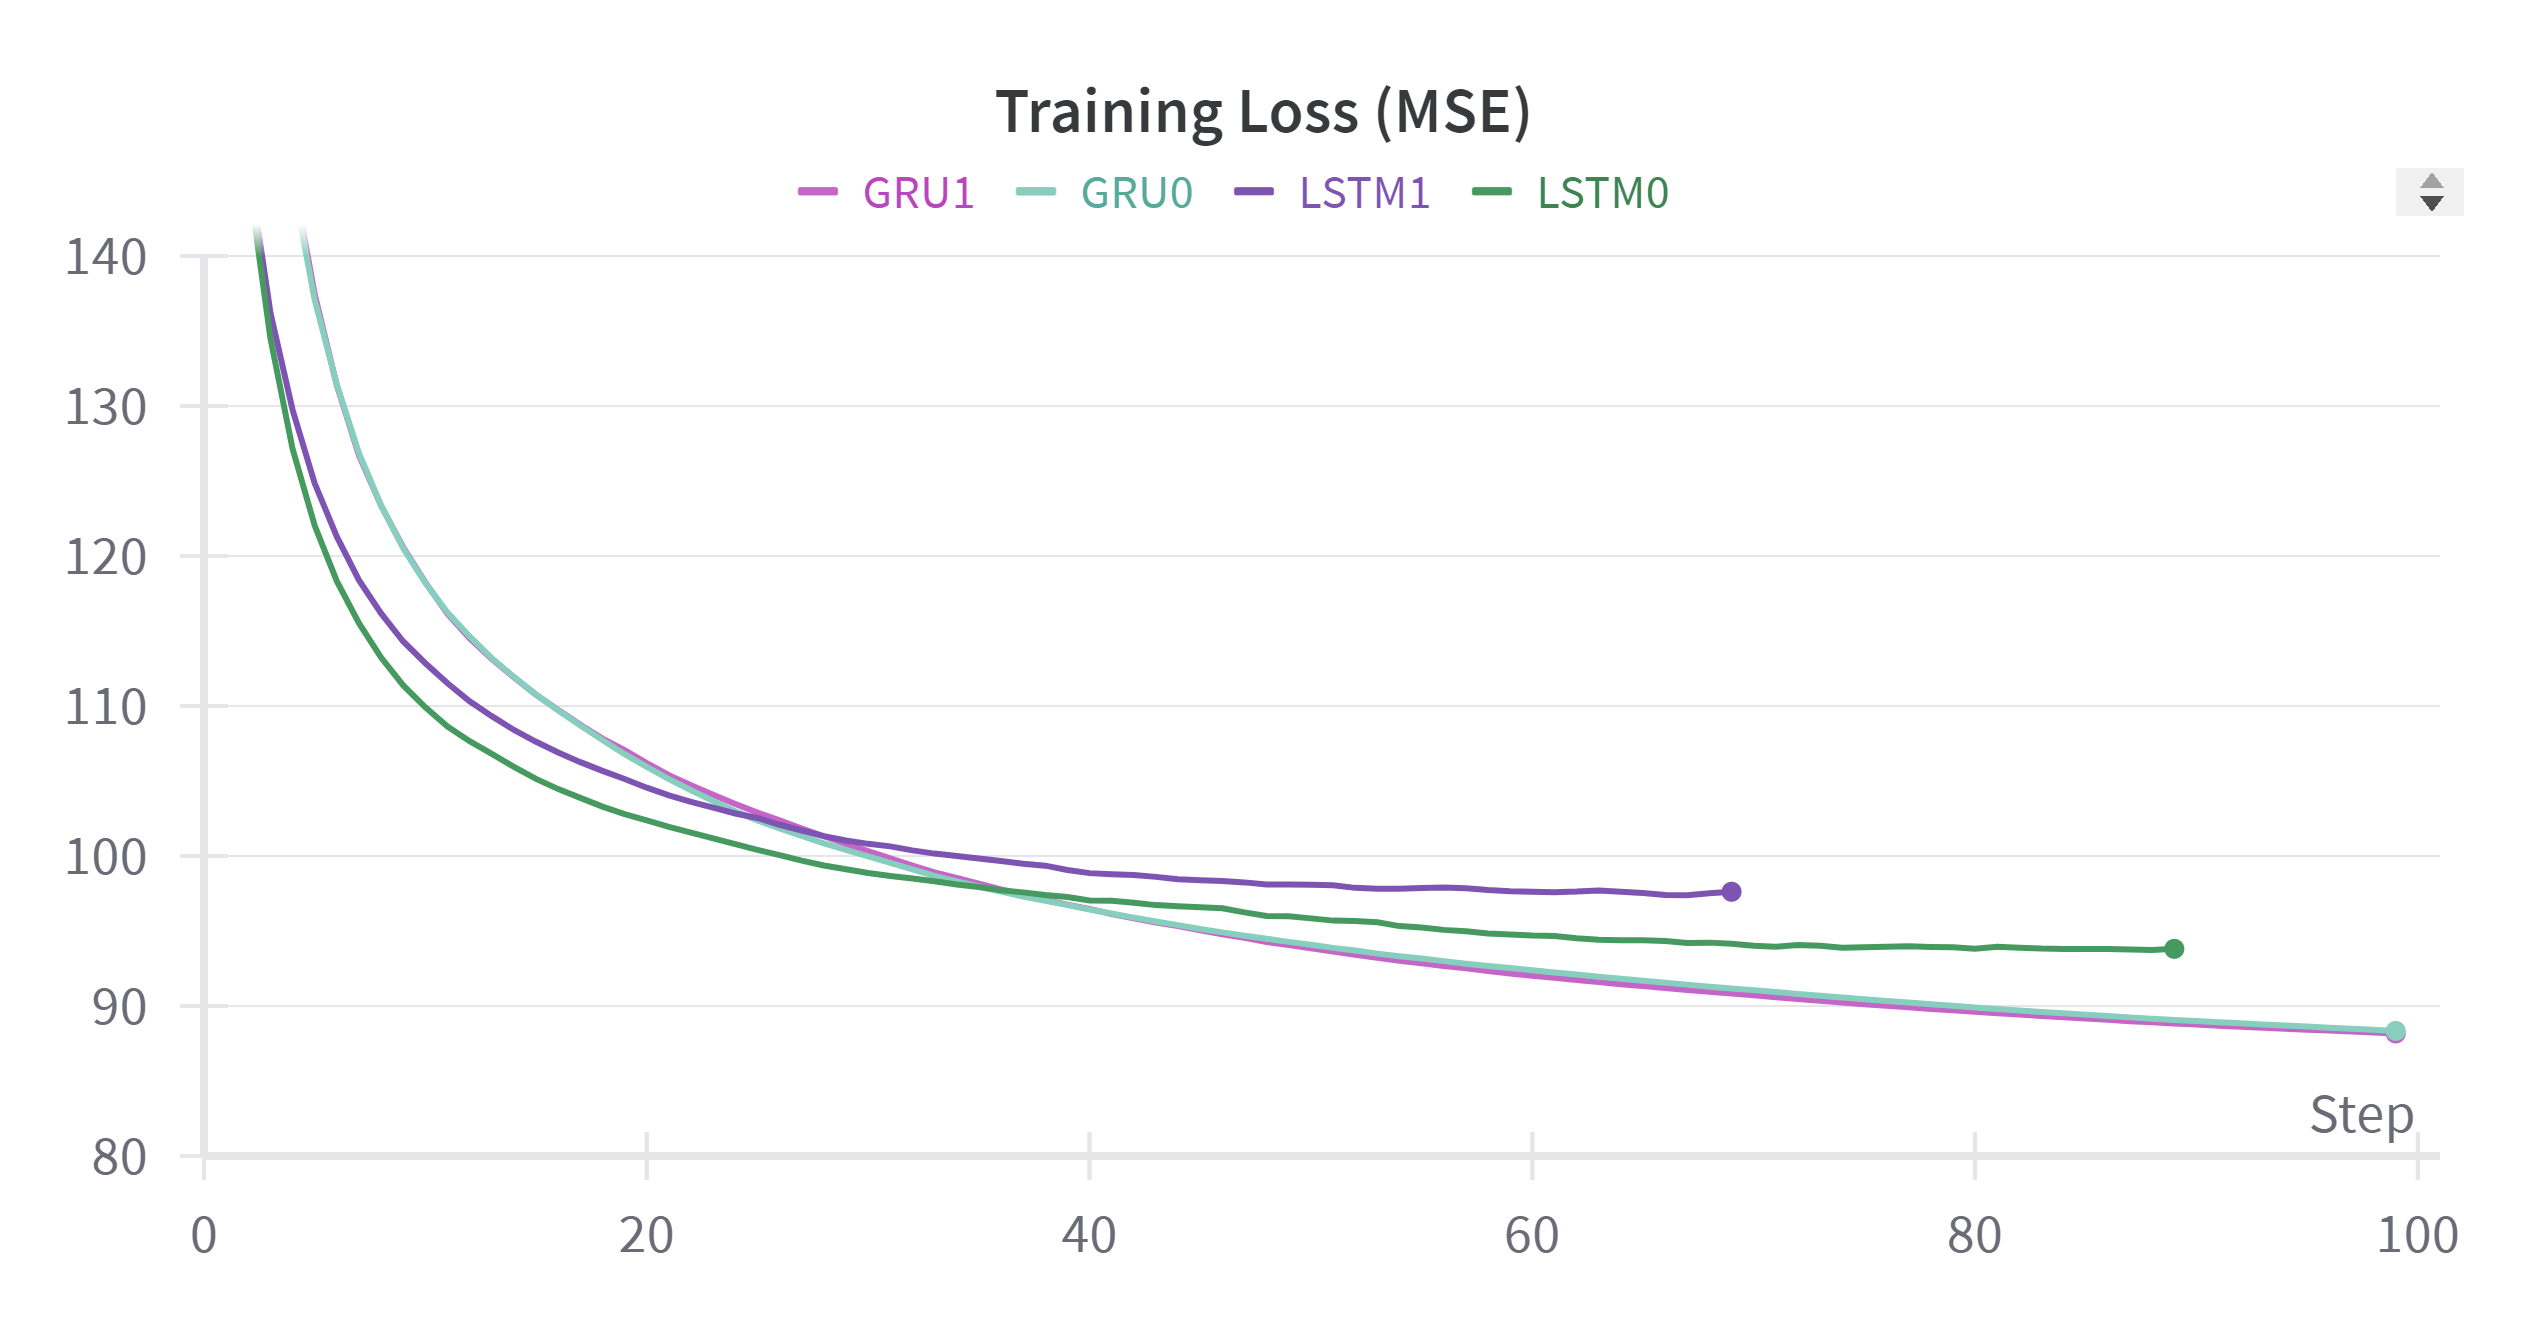
\includegraphics[width=0.4\linewidth]{images/results/LSTM_GRU_Train_mse}
%        \caption{LSTM \& GRU Train MSE}
%        \label{fig:train_mse}
%    \end{subfigure}
%    \begin{subfigure}{0.5\textwidth}
%        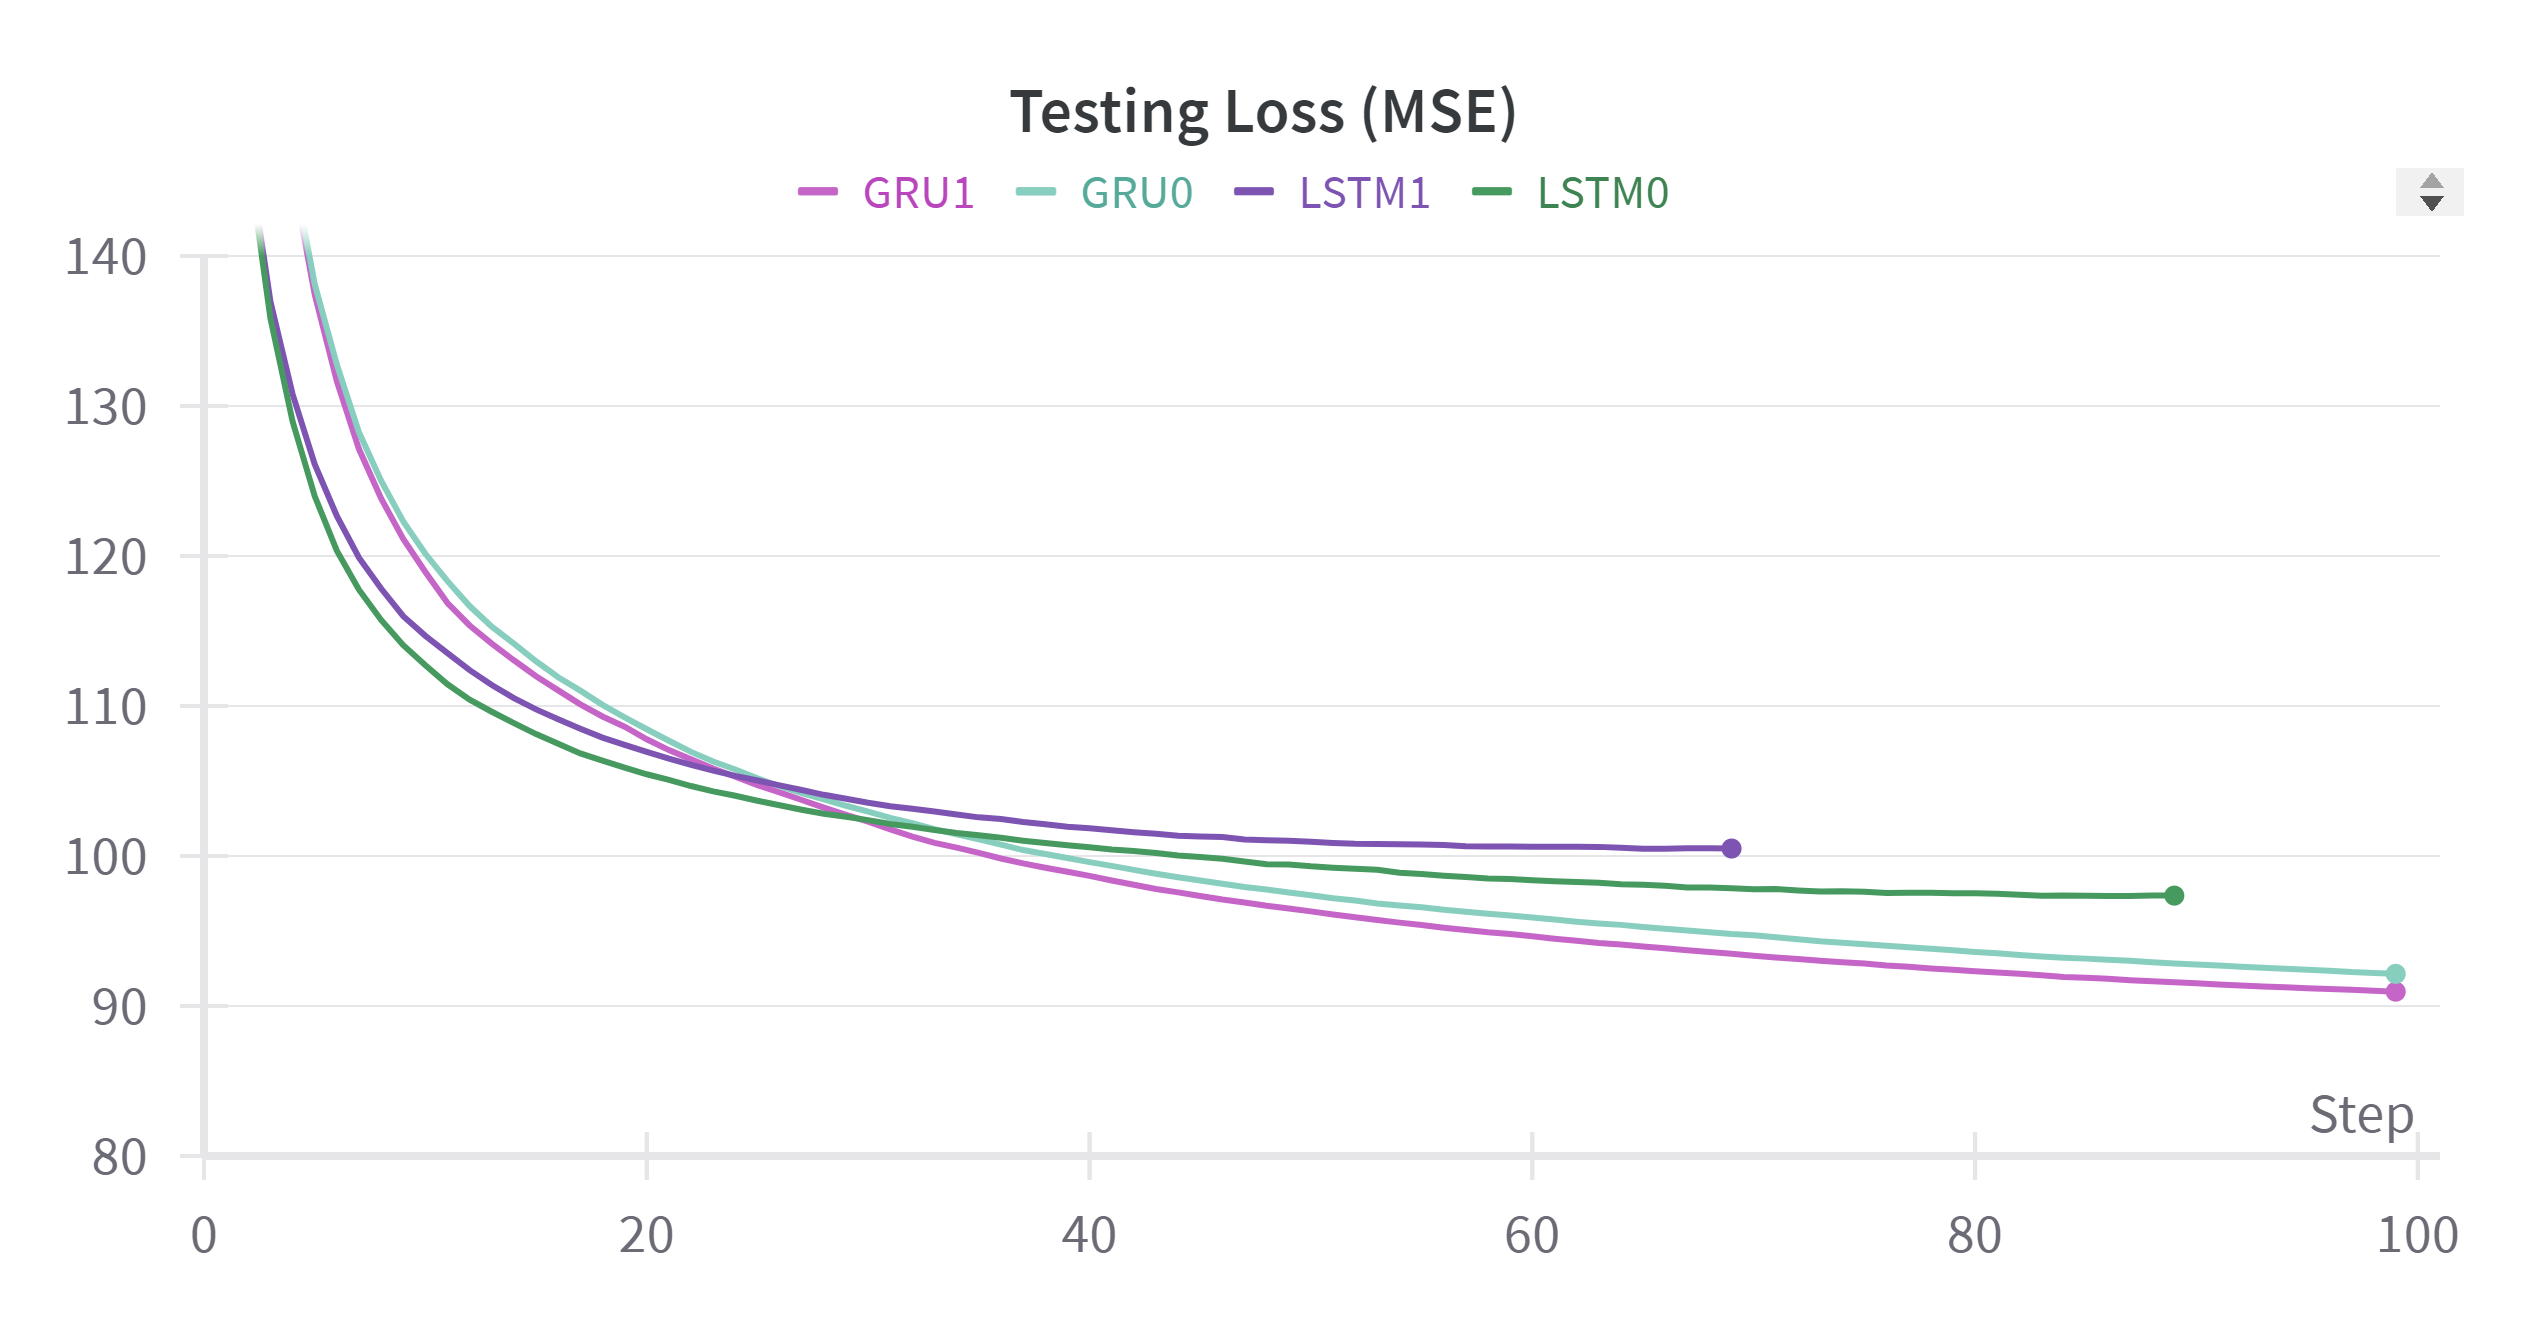
\includegraphics[width=0.4\linewidth]{images/results/LSTM_GRU_Test_mse}
%        \caption{LSTM \& GRU Test MSE}
%        \label{fig:test_mse}
%    \end{subfigure}
%\end{figure}

\begin{figure}[h]
    \centering
    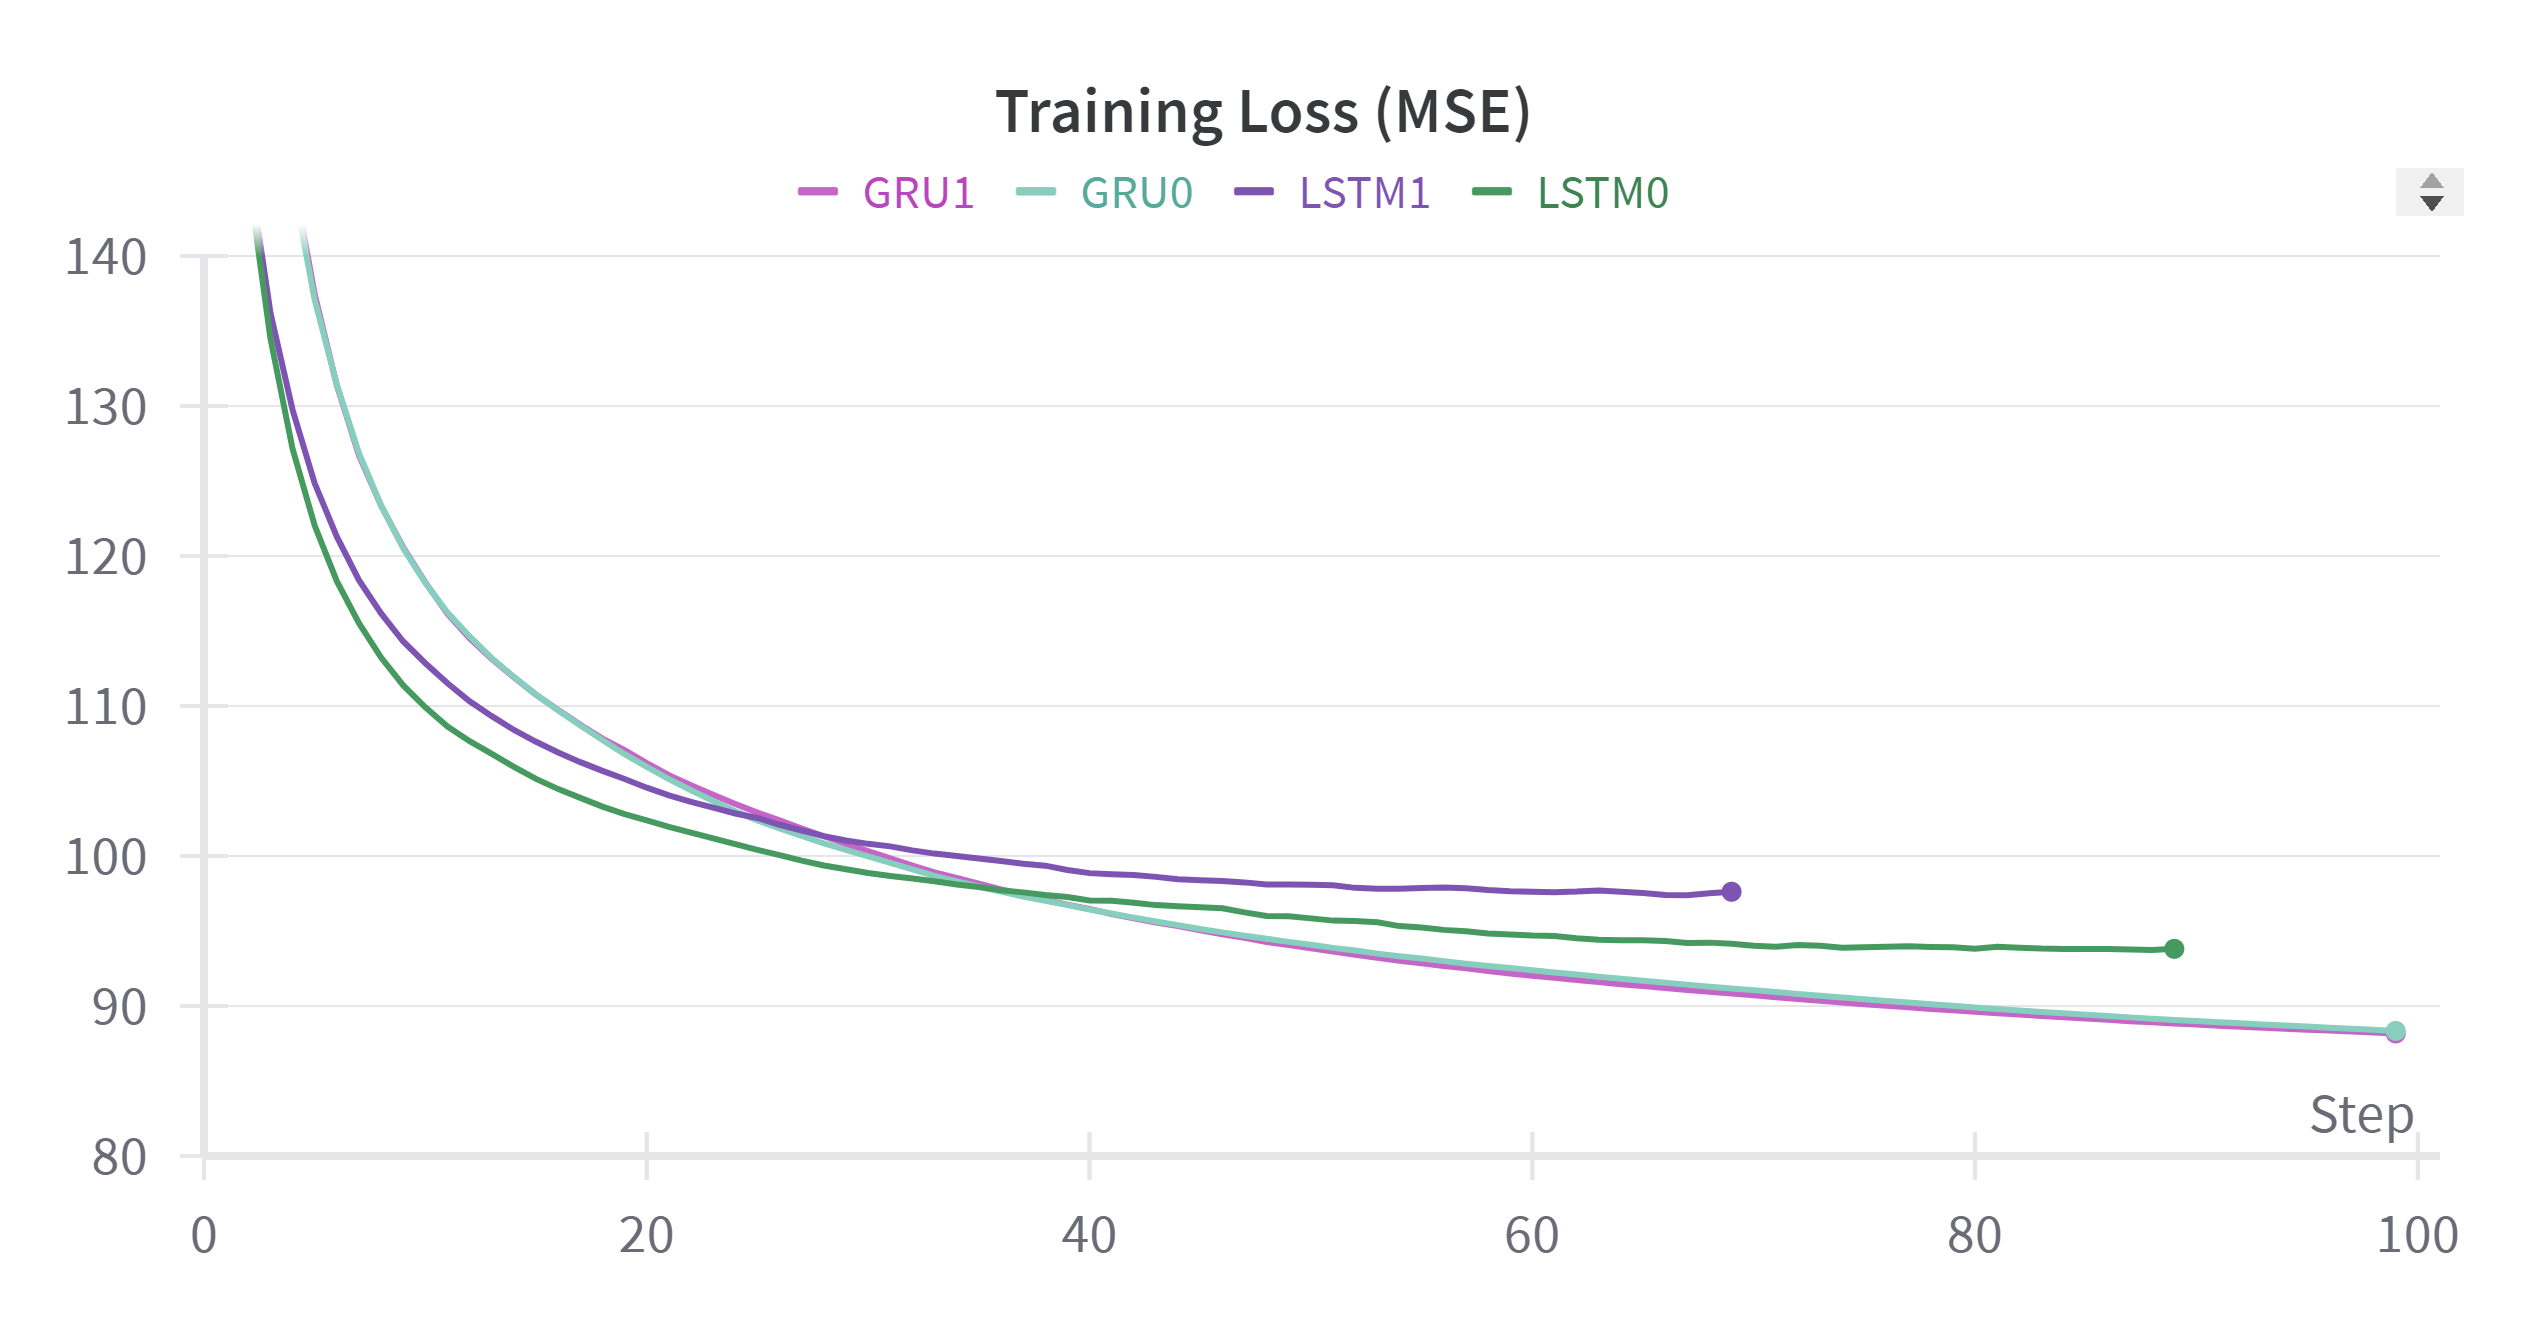
\includegraphics[width=0.4\linewidth]{images/results/LSTM_GRU_Train_mse}
    \caption{LSTM \& GRU Train MSE}
    \label{fig:train_mse}
\end{figure}

\begin{figure}[h]
    \centering
    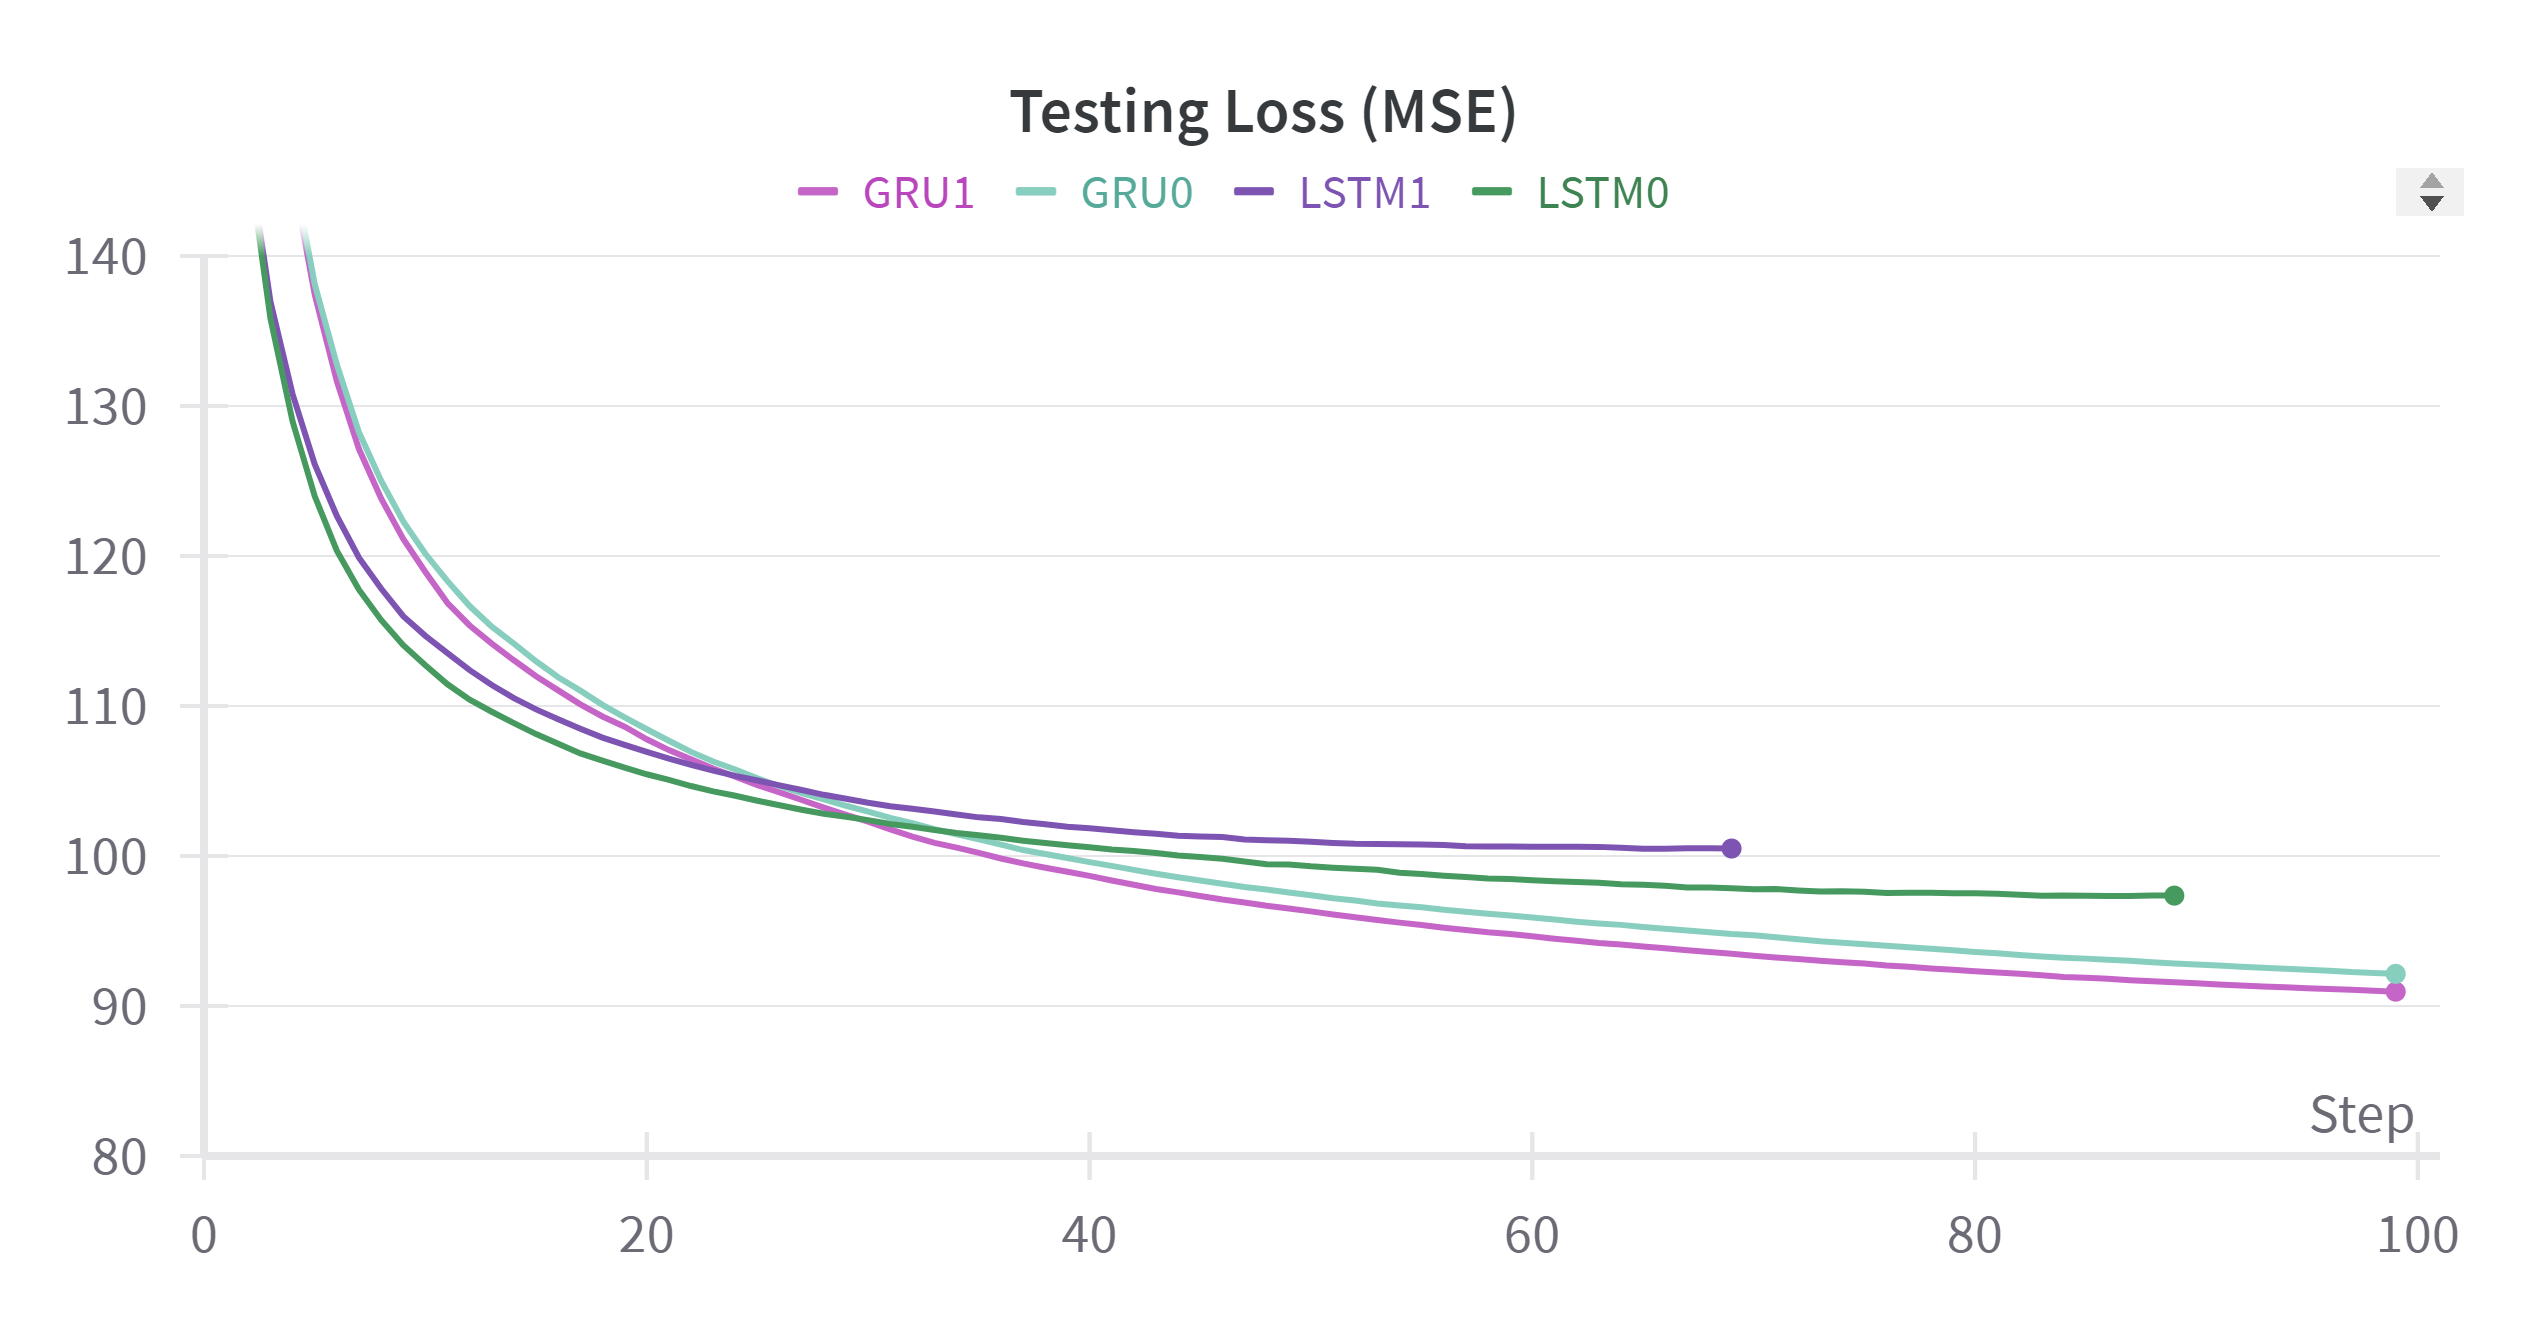
\includegraphics[width=0.4\linewidth]{images/results/LSTM_GRU_Test_mse}
    \caption{LSTM \& GRU Test MSE}
    \label{fig:test_mse}
\end{figure}

\begin{figure}[h]
    \centering
    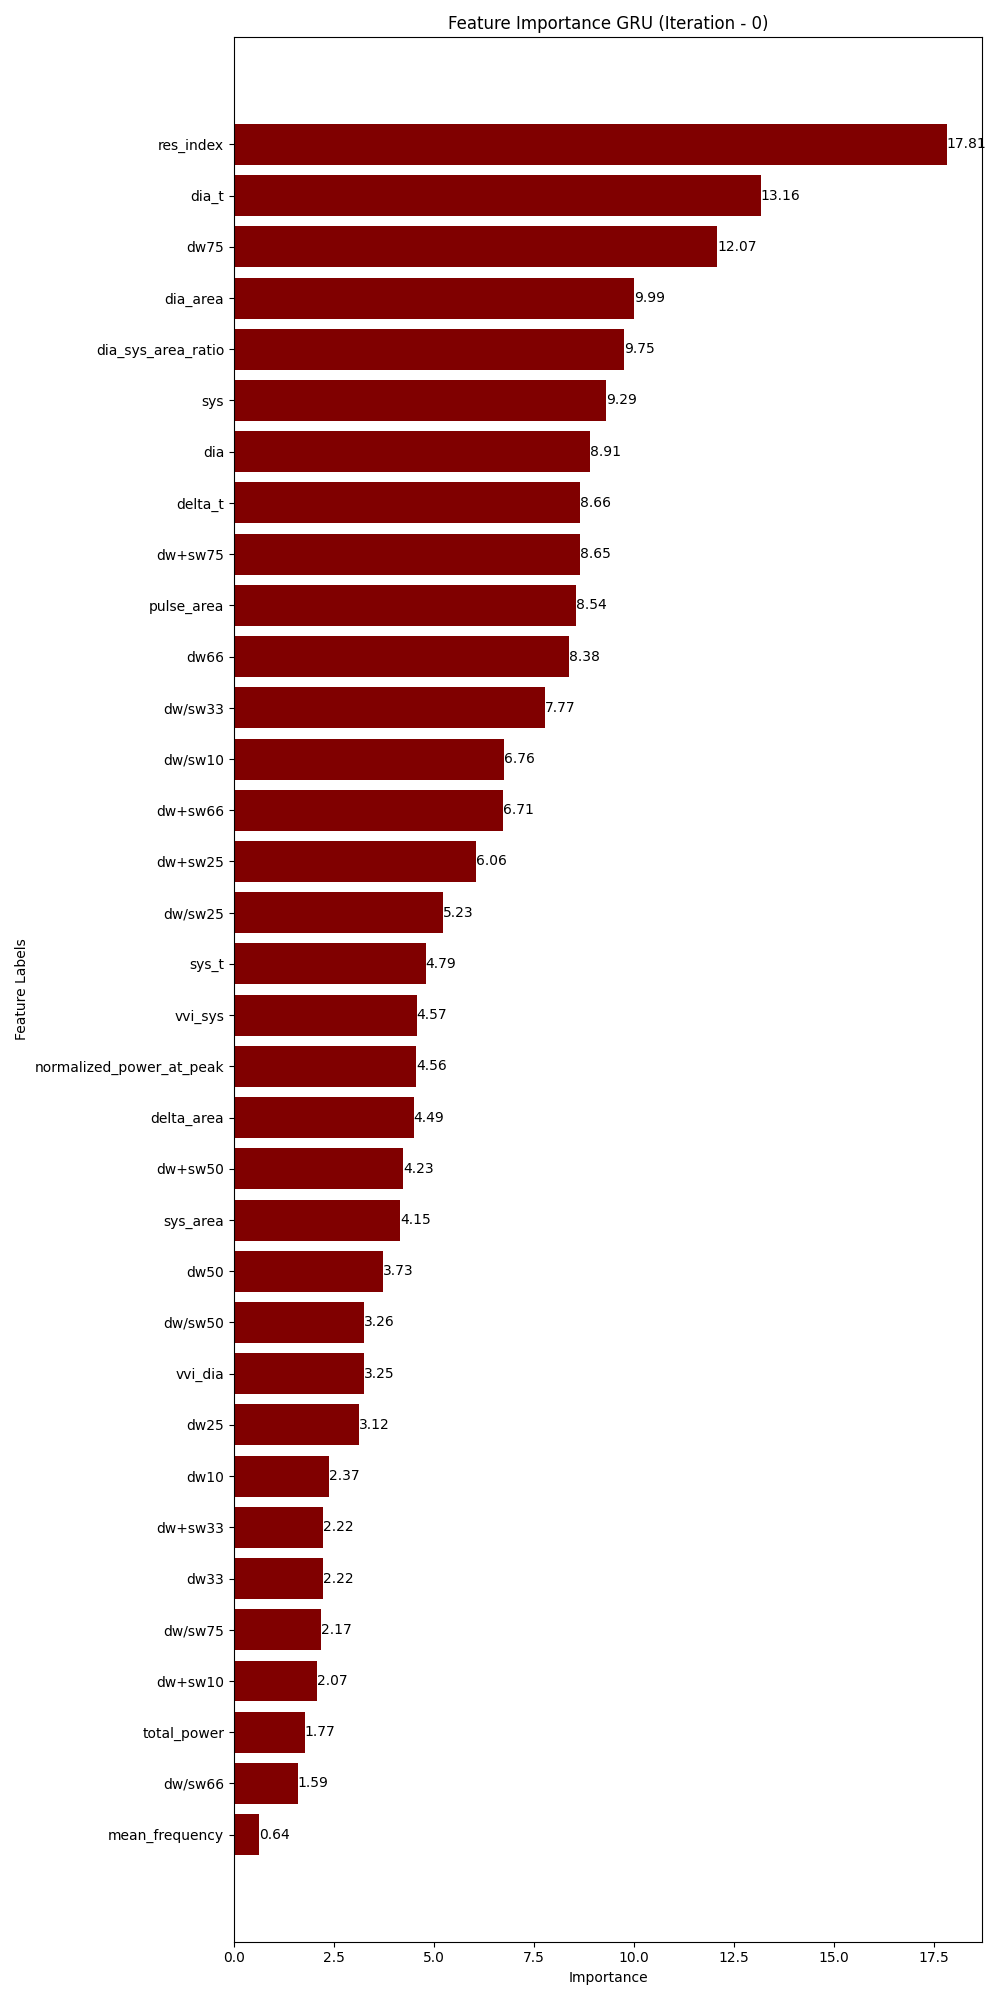
\includegraphics[width=0.5\textwidth]{images/results/feature_importance_plot_GRU_0}
    \caption{Feature Importance Chart}
    \label{fig:feat_importance}
\end{figure}
